\documentclass[a4paper,12pt]{article}
\usepackage[slovene]{babel}
\usepackage[utf8]{inputenc}
\usepackage[T1]{fontenc}
\usepackage{lmodern}
\usepackage{amsmath,amsfonts}
\usepackage{enumitem}
\usepackage{graphicx}
\usepackage{subfigure}
\pagenumbering{roman}

\begin{document}

\newcommand{\N}{\mathbb{N}}
\newcommand{\R}{\mathbb{R}}
\newcommand\sbullet[1][.5]{\mathbin{\vcenter{\hbox{\scalebox{#1}{$\bullet$}}}}}


\title{Diskretne Coonsove ploskve}
\author{Matej Rojec, Vito Rozman}
\date{\today}

\maketitle


\newpage

\tableofcontents
\listoffigures

\newpage

\section{Uvod in motivacija}

\subsection{Uvod v Bézierjeve ploskeve}
Bézierjevo ploskev $\mathbf{p} : [0,1]^2 \rightarrow \R^3$ iz tenzorskega produkta stopnje $(m, n) \in \N \times \N$  
definiramo s parametrizacijo:
$$\mathbf{p}(u,v) := \sum_{i=0}^m \sum_{j=0}^n \mathbf{b}_{i,j} B_i^m(u)B_j^n(v),$$
kjer sta $u,v$ iz enotskega kvadrata, t.j $(u,v) \in [0,1]^2$ ter $(\frac{i}{m}, \frac{j}{n})$
domenske točke, ki ustrezajo kontrolni točki $\mathbf{b}_{i,j}$.

Pri fiksnem $v$, množica $\{\mathbf{b} (u,v) \mid u \in [0,1]  \}$ predstavlja 
kontrolnimi točkami
$$\sum_{j=0}^n \mathbf{b}_{i,j} B_j^n(v), \qquad i=0,1,\ldots,m,$$
ki so izračunane kot točke na Bézierjevih krivuljah stopnje $n$ pri parametru $v$.


\subsection{Coonsove ploskve}

Denimo, da imamo podane kontrole točke $\mathbf{b}_{i,j},~ i=0,\ldots,m,~ j=0,\ldots,n$.
Te določajo štiri robne krivulje 
Te omejujejo iskano ploskev $\mathbf{p}$ iz tenzorskega produkta stopnje $(n,m)$.
Kontrolne točke
\begin{align*}
      &\mathbf{b}_{0,0} &\mathbf{b}_{1,0} & &\ldots & &\mathbf{b}_{m-1,0} & &\mathbf{b}_{m,0} \\
      &\mathbf{b}_{0,1}  &  & &  & &  & &\mathbf{b}_{m,1} \\
      &\vdots  &  &  & &  & & &\vdots\\
      &\mathbf{b}_{0,n-1}  &  &  & &  & &  &\mathbf{b}_{m,n-1} \\ 
      &\mathbf{b}_{0,n} &\mathbf{b}_{1,n} & &\ldots & &\mathbf{b}_{m-1,n} & &\mathbf{b}_{m,n} \\
\end{align*}
določajo štiri Bézierjev krivulje: 
\begin{align*}
   &\mathbf{p}(u,0) =\sum_{i=0}^m \mathbf{b}_{i,0} B_i^n(u),  \\
   &\mathbf{p}(u,1) =\sum_{i=0}^m \mathbf{b}_{i,n} B_i^n(u),  \\
   &\mathbf{p}(0,v) =\sum_{j=0}^n \mathbf{b}_{0,j} B_j^n(v),  \\
   &\mathbf{p}(1,v) =\sum_{j=0}^n \mathbf{b}_{m,j} B_j^n(v),  \\
\end{align*}
kjer je domena enotski kvadrat, t.j.~$(u,v) \in [0,1]^2$.
Kontrolne točke torej omejujejo ploskev $\mathbf{p}$. 
Sedaj potrebujemo definirati še ostale kontrolne točke 
$\mathbf{b}_{i,j},~ i=1,\ldots, m-1~, j=1,\ldots,n-1$. 
V ta namen definiramo tri dodatne ploskve:
\begin{enumerate}
   \item Prva je Bézierjeva ploskev stopnje $(m, 1)$, ki je kot ploskev stopnje $(m,n)$ podana s kontrolnimi točkami:
   $$\mathbf{b}_{i,j}^{(1)} = \left(1-\frac{j}{n}  \right) \mathbf{b}_{i,0} + \frac{j}{n} \mathbf{b}_{i,n} $$
   \item Druga je Bézierjeva ploskev stopnje $(1, n)$, ki je kot ploskev stopnje $(m,n)$ podana s kontrolnimi točkami:
   $$\mathbf{b}_{i,j}^{(2)} = \left(1-\frac{i}{m}  \right) \mathbf{b}_{0,j} + \frac{i}{m} \mathbf{b}_{m,j} $$
   \item Tretja je Bézierjeva ploskev stopnje $(1, 1)$, ki je kot ploskev stopnje $(m,n)$ podana s kontrolnimi točkami:
   $$
   \mathbf{b}_{i,j}^{(3)} = \left(1-\frac{i}{m}  \right) \left(1-\frac{j}{n}  \right) \mathbf{b}_{0,0} 
         + \frac{i}{m} \left(1-\frac{j}{n}  \right) \mathbf{b}_{m,0}
         + \left(1-\frac{i}{m}  \right) \frac{j}{n}  \mathbf{b}_{0,n} 
         + \frac{i}{m} \frac{j}{n} \mathbf{b}_{m,n} 
   $$
\end{enumerate}
Coonsova ploskev $\mathbf{p}$ je definirana s kontrolnimi točkami 
$$\mathbf{b}_{i,j} := \mathbf{b}_{i,j}^{(1)}+\mathbf{b}_{i,j}^{(2)}+\mathbf{b}_{i,j}^{(3)}.$$
Primer krivulje je prikazan na sliki \ref{fig:whatever}. 
Prikazane so robne točke ter ogrodje kontrolnih točk, ki jih dobimo iz teh 
robnih točk in krivulja na danem ogrodju.

\begin{figure}[ht!]
   \centering
   \subfigure[Primer robnih točk]{
   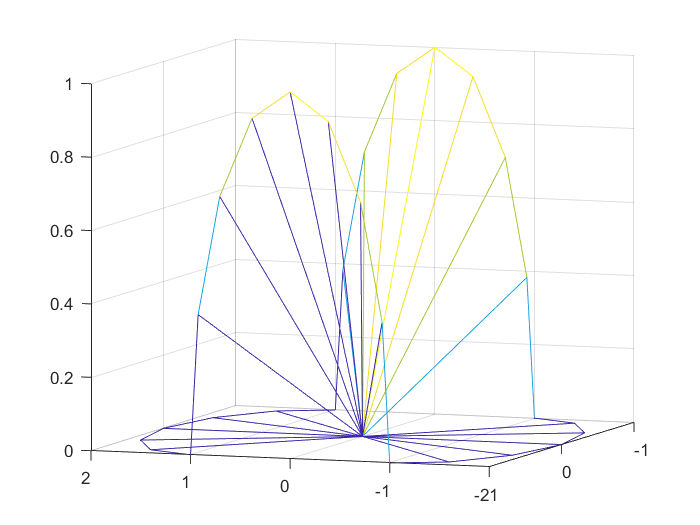
\includegraphics[width=0.45\textwidth]{ogrodje.png}
   }
   \subfigure[Primer ogrodja]{
   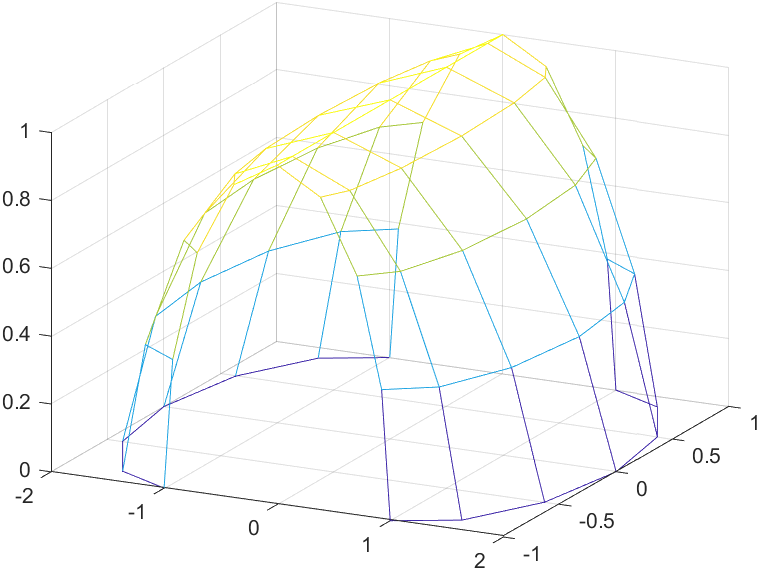
\includegraphics[width=0.45\textwidth]{dodatne_kont_t.png}
   }
   
   \subfigure[Coonsova ploskv na ogrodju]{
   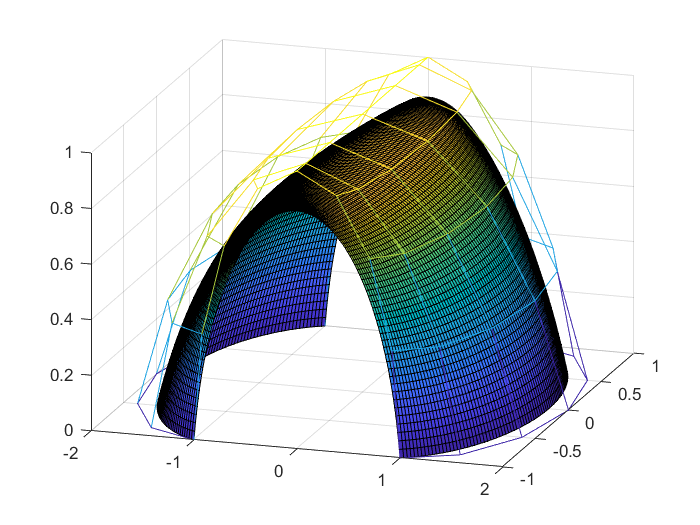
\includegraphics[width=0.5\textwidth]{primer_krivulje.png}
   }   
   \caption{Primer konstrukcije Coonsove ploskve}
\label{fig:whatever}
\end{figure}
Iz slike \ref{fig:whatever} opazimo, da so ploskev zelo ravna. Več o tem bomo komentirali kasneje.

\section{Lastnosti Coonsovih ploskev}

\subsection{Minimziraje zasuka}
Coonsova ploskve minimzirajo zasuk, definiran kot:
\begin{equation}
   \label{eq:min}
   \int_{[0,1]^2} \left( \frac{\partial^2}{\partial u \partial v}\mathbf{p}(u,v) \right)^2 dS.
\end{equation}
Torej coonsova ploskev doseže minimum izraza \eqref{eq:min}.
Posledica tega je, da so Coonsova ploskve lahko v primerih preveč ravne in ne interpolirajo dobro kontrolnih točk.
Taka ploskev prav tako zadošča Euler-Lagrangovi parcialni diferencialni enačbi, torej velja:
\begin{equation}
   \label{eq:pde}
    \frac{\partial^4}{\partial u^2 \partial v^2}\mathbf{p}(u,v) = 0.
\end{equation}

\subsection{Ohranjanje Coonsove ploskve}

Izberimo dve točki $(u_0, v_0)$ ter $(u_1,v_1)$, ki definirajo pravokotnik $P$
v domeni $[0,1]^2$ Coonsove ploskve. 
Robovi pravokotnika $P$ definirajo štiri robne krivulje.
Sedaj tvorimo novo Coonsovo ploskev podano z robnimi krivuljami pravokotnika $P$.
Ta ploskev je enaki Coonsovi ploskvi prvotne krivulje zožane na pravokotnik $P$.

Predpostavimo, da imamo podano ploskev $\mathbf{p}$ iz tenzorskega produkta stopnje $(n,m)$.
Oglejmo si poljubno $3\times 3$ podmrežo podano kot:
\begin{align*}
      &\mathbf{b}_{i-1,j-1} &\mathbf{b}_{i,j-1}& &\mathbf{b}_{i+1,j-1} \\
      &\mathbf{b}_{i-1,j} &\mathbf{b}_{i,j}& &\mathbf{b}_{i+1,j}. \\
      &\mathbf{b}_{i-1,j+1} &\mathbf{b}_{i,j+1}& &\mathbf{b}_{i+1,j+1} \\ 
\end{align*}
V primeru, da poznamo robne točke $3\times 3$ mreže, lahko po zgoraj povedanem
notranjo točko $\mathbf{b}_{i,j}$ izačunamo kot:
\begin{align*}
   \mathbf{b}_{i,j} =&-\frac{1}{4}(\mathbf{b}_{i-1,j-1}+\mathbf{b}_{i+1,j-1}+\mathbf{b}_{i-1,j+1}+\mathbf{b}_{i+1,j+1}) \\
   &+\frac{1}{2}(\mathbf{b}_{i,j-1}+\mathbf{b}_{i-1,j}+\mathbf{b}_{i+1,j}+\mathbf{b}_{i,j+1}).\\
\end{align*}
To lahko zapišemo s pomočjo t.i. maske kot:
\begin{align*}
                                        & &-1  & &2 & &-1 \\
   &\mathbf{b}_{i,j}=\frac{1}{4} \times & 2 & & \sbullet & & 2 .\\
                                        & &-1 & &2 & &-1 \\ 
\end{align*}
Mreža je sestavljena iz $(m+1)\times(n+1)$ kontrolnih točk, od teh ne poznamo 
$(m-1)\times(n-1)$ izmed njih. 
Za vsako izmed $(m-1)\times(n-1)$ imamo natanko eno enačbo, ki je določena z zgoraj opisano masko.
To je seveda zelo časovno zahtevna metoda, da izračunamo kontrolne točke Coonsove ploskve,
ampak nam da nov vpogled, kako bi lahko izračunali kontrolne točke Coonsove ploskve.
Vidimo, da so kontrolne točke Coonsove ploskve poseben primer maske oblike:
\begin{align*}
   & &\alpha  & &\beta & &\alpha \\
&\mathbf{b}_{i,j}= \times & \beta & & \sbullet & & \alpha,\\
   & &\alpha & &\beta & &\alpha \\ 
\end{align*}
kjer je $(\alpha, \beta) = (-0.25, 0.5)$. To nam, da idejo da bi lahko izbrali različne 
parametra $\alpha$ in $\beta$ sprmenili. Vedno bomo privzeli, da velja $4\alpha + 4\beta = 1$.
\end{document}